\localauthor{Stefanie Gürster}
\subsection{Wireframe}

Die Grundstruktur der Applikation wird in Abbildung \ref{fig:wireframe} abbgebildet, welche sich auch in den folgenden Mockups in Abbildung \ref{fig:homepageMockup} und in Abbildung \ref{fig:submission} wiederspiegelt.
Inhalte mit gestrichelten Linen sind dabei nicht immer in jeder Ansicht sichtbar.

\begin{figure}[H]
	\centering
	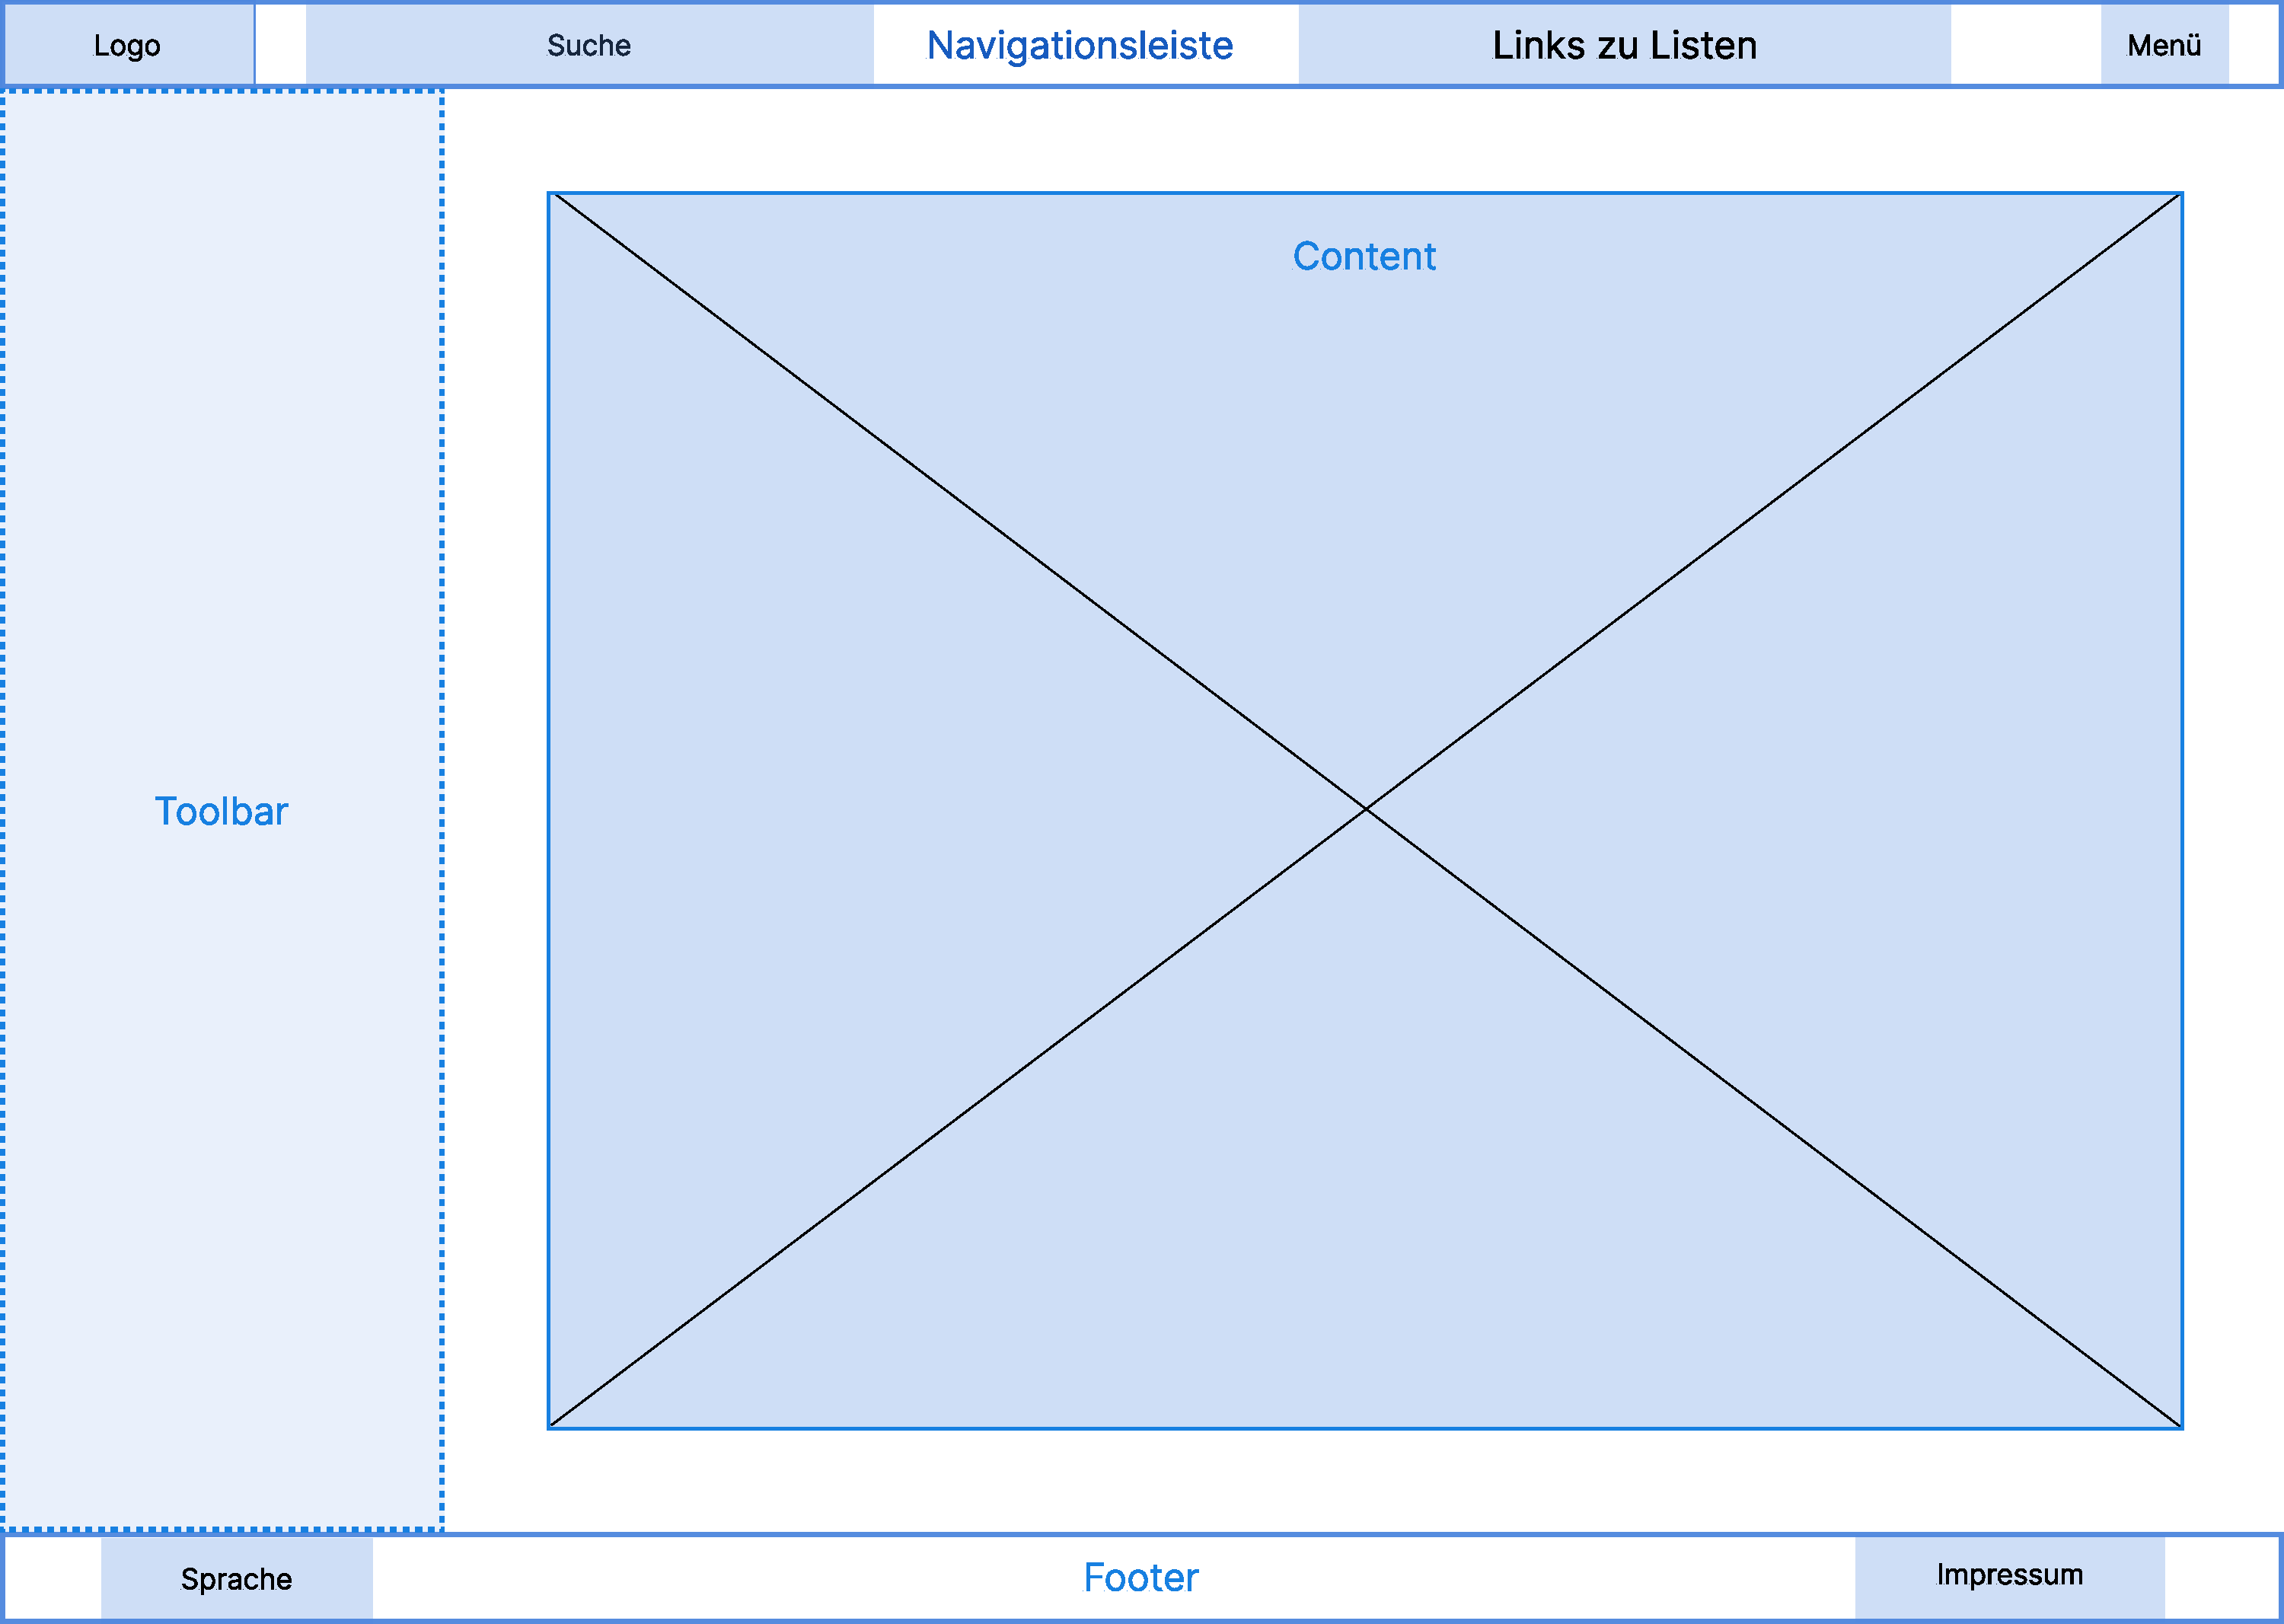
\includegraphics[width=0.85\linewidth]{graphics/Wireframe}
	\caption{Grundstruktur der Applikation}
	\label{fig:wireframe}
\end{figure}

\subsection{Mockups}

Folgende Bilder zeigen einen Prototyp der Anwendung.
Dargestellt sind zwei Ausschnitte aus Schlüsselfunktionen der Webanwendung.

Die Startseite in Abbildung \ref{fig:homepageMockup} ist auf die Rolle eines \hyperref[glo:editor]{Editors} zugeschnitten, wobei dieser auch einige
Reviews bearbeitet und somit auch die Rolle des \hyperref[glo:gutachter]{Gutachters} für einige Einreichungen bekleidet.
Je nach ausgewähltem Reiter erscheinen entweder eigene, zu begutachtende Einreichungen oder Einreichungen die in eigener editorialer Verantwortung liegen.

Die Übsersichtsseite der Einreichung, die Submission Site, in Abbildung \ref{fig:submission} ist ebenfalls auf die Rolle eines \hyperref[glo:editor]{Editors} ausgelegt.
Ihm steht im Gegensatz zu einem \hyperref[glo:regnutzer]{normalen Nutzer}, welcher keine ander Rolle bekleidet, eine Toolbar zur Verfügung.
Mithilfe dieser kann er Gutachter verwalten, einen anderen \hyperref[glo:editor]{Editor} ernennen oder eine Revision anfordern.


\subsubsection{Startseite}

\begin{figure}[H]
	\centering
	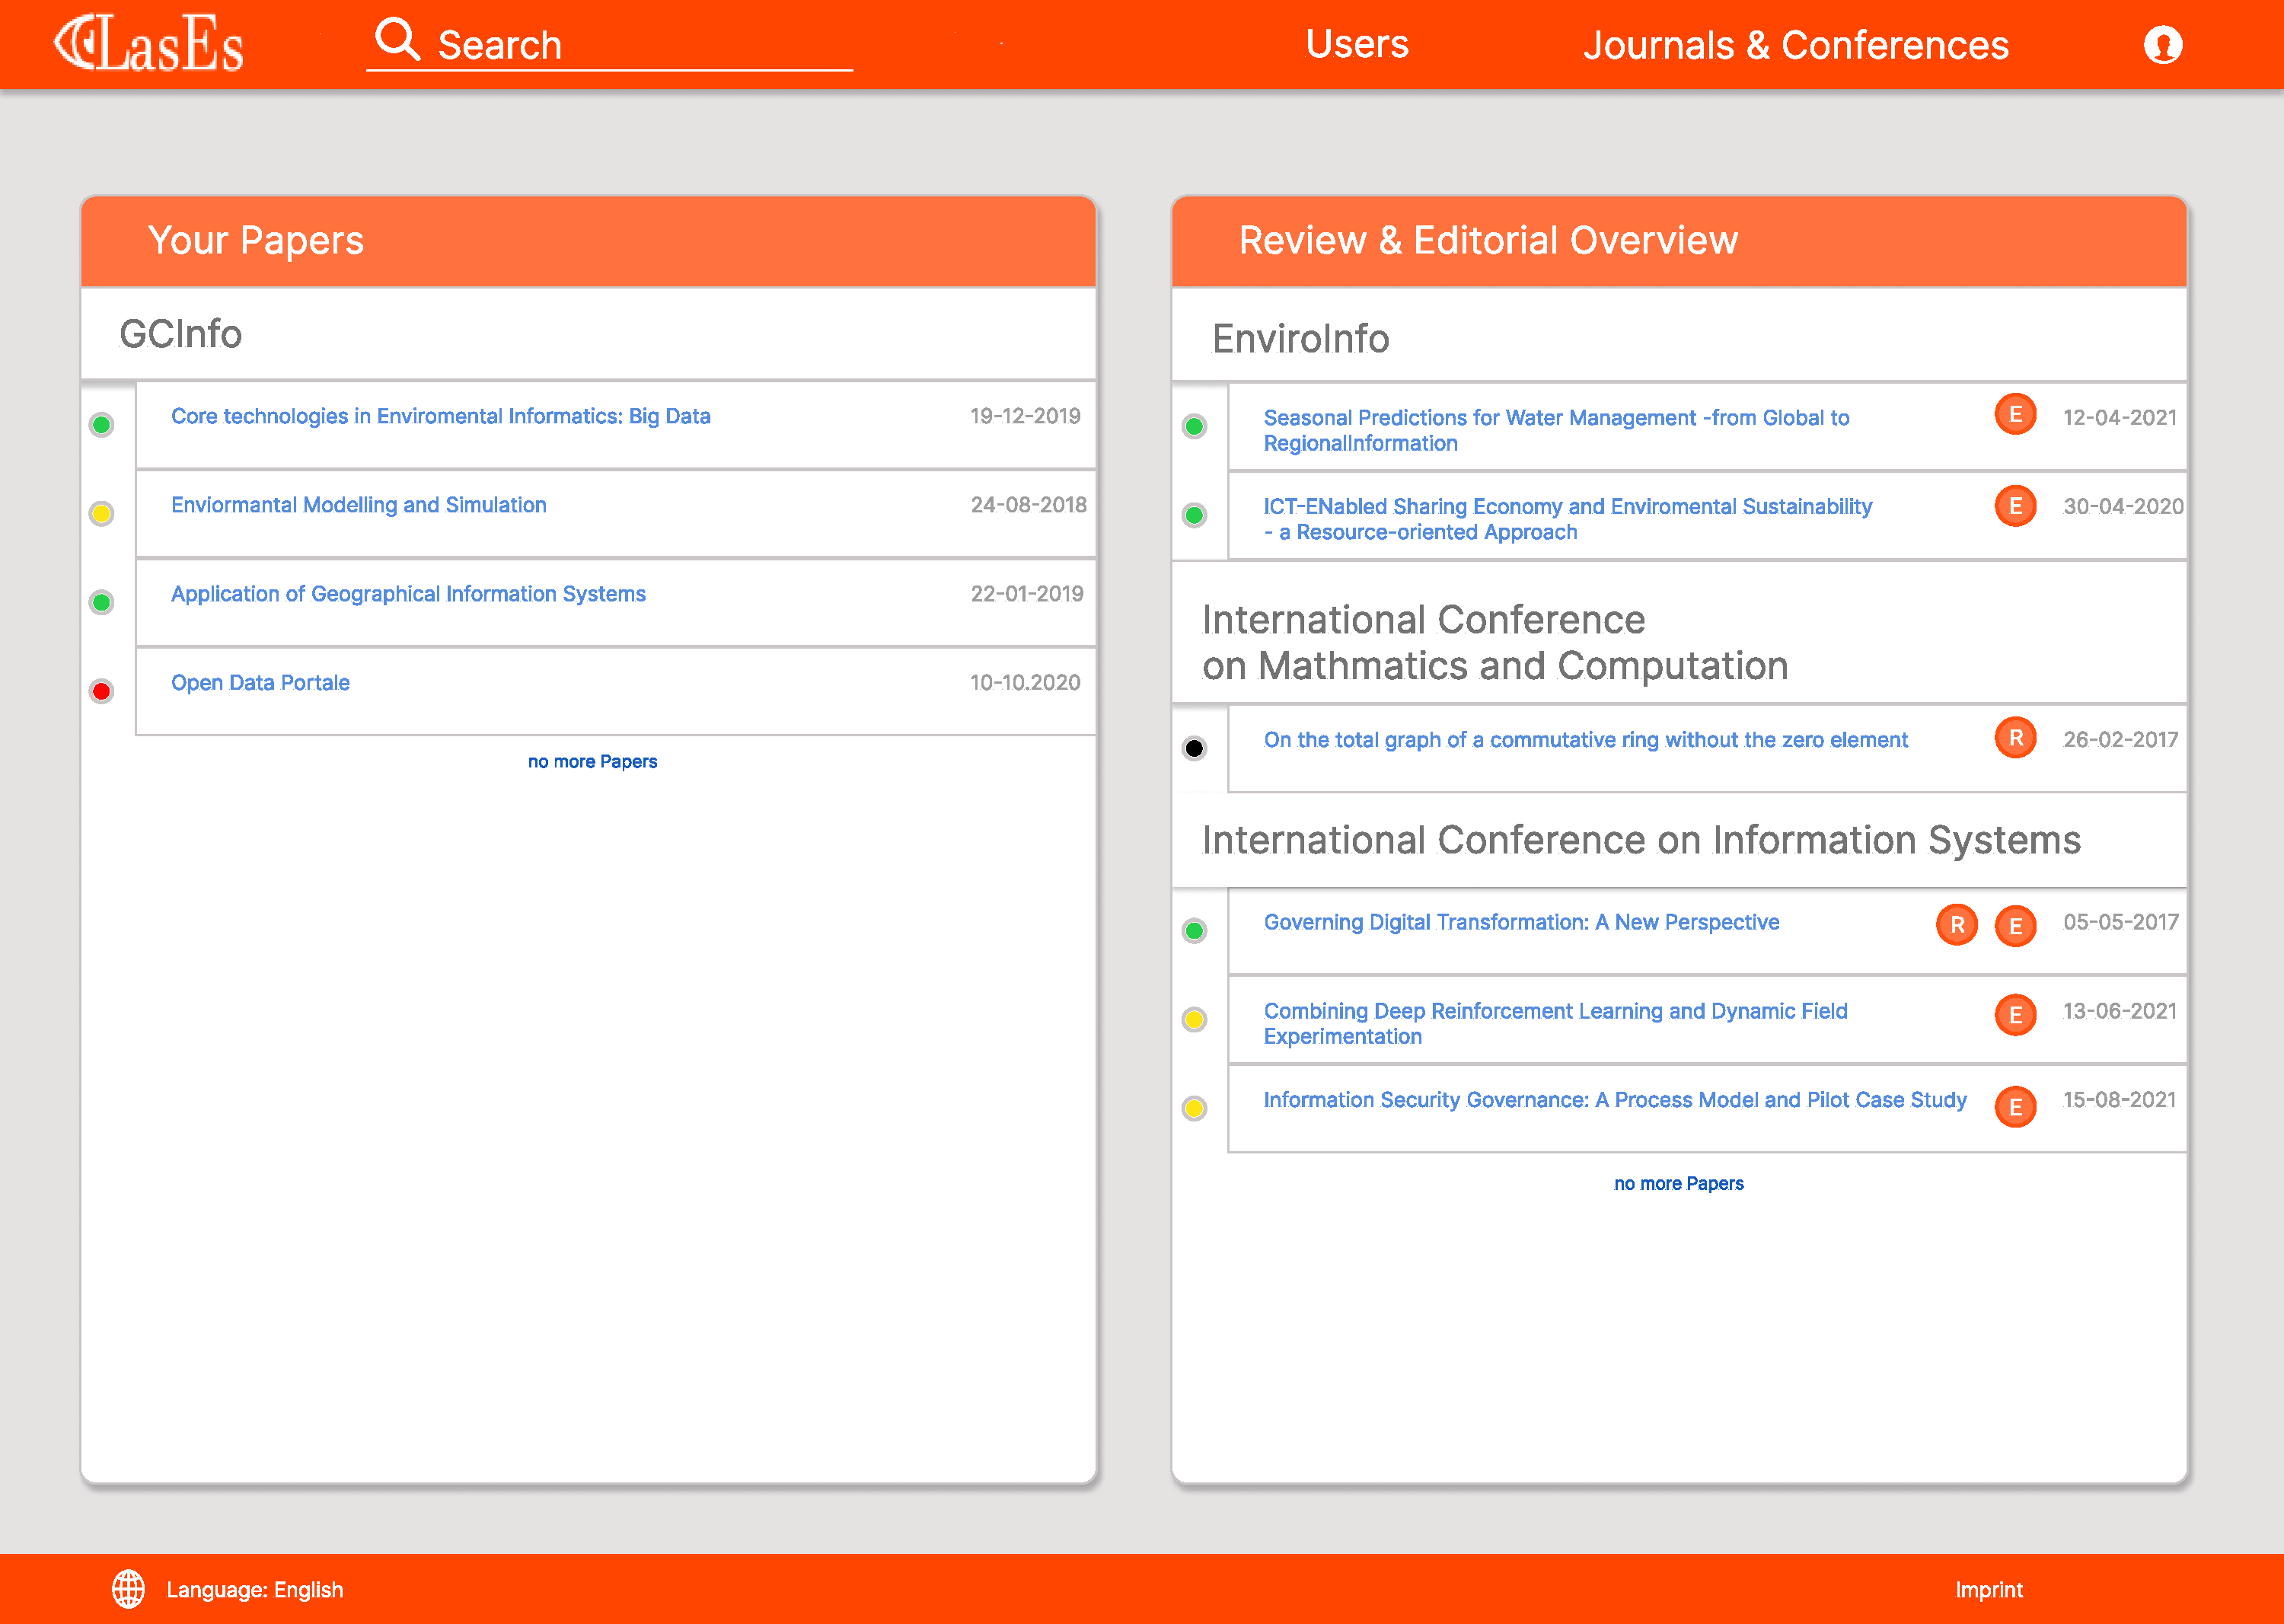
\includegraphics[width=0.85\linewidth]{graphics/Homepage}
	\caption{Übersicht auf einer Startseite}
	\label{fig:homepageMockup}
\end{figure}

\subsubsection{Submission}

\begin{figure}[H]
	\centering
	\includegraphics[width=0.85\linewidth]{graphics/Submission}
	\caption{Ablauf einer erfolgreichen Einreichung nach Reviews}
	\label{fig:submission}
\end{figure}


\subsection{Benutzerfluss}
Im Folgenden werden functioning Aussagen über die Benutzeroberfläche mithilfe eines Benutzerflussdiagramms getroffen.

\begin{figure}[H]
    \centering
    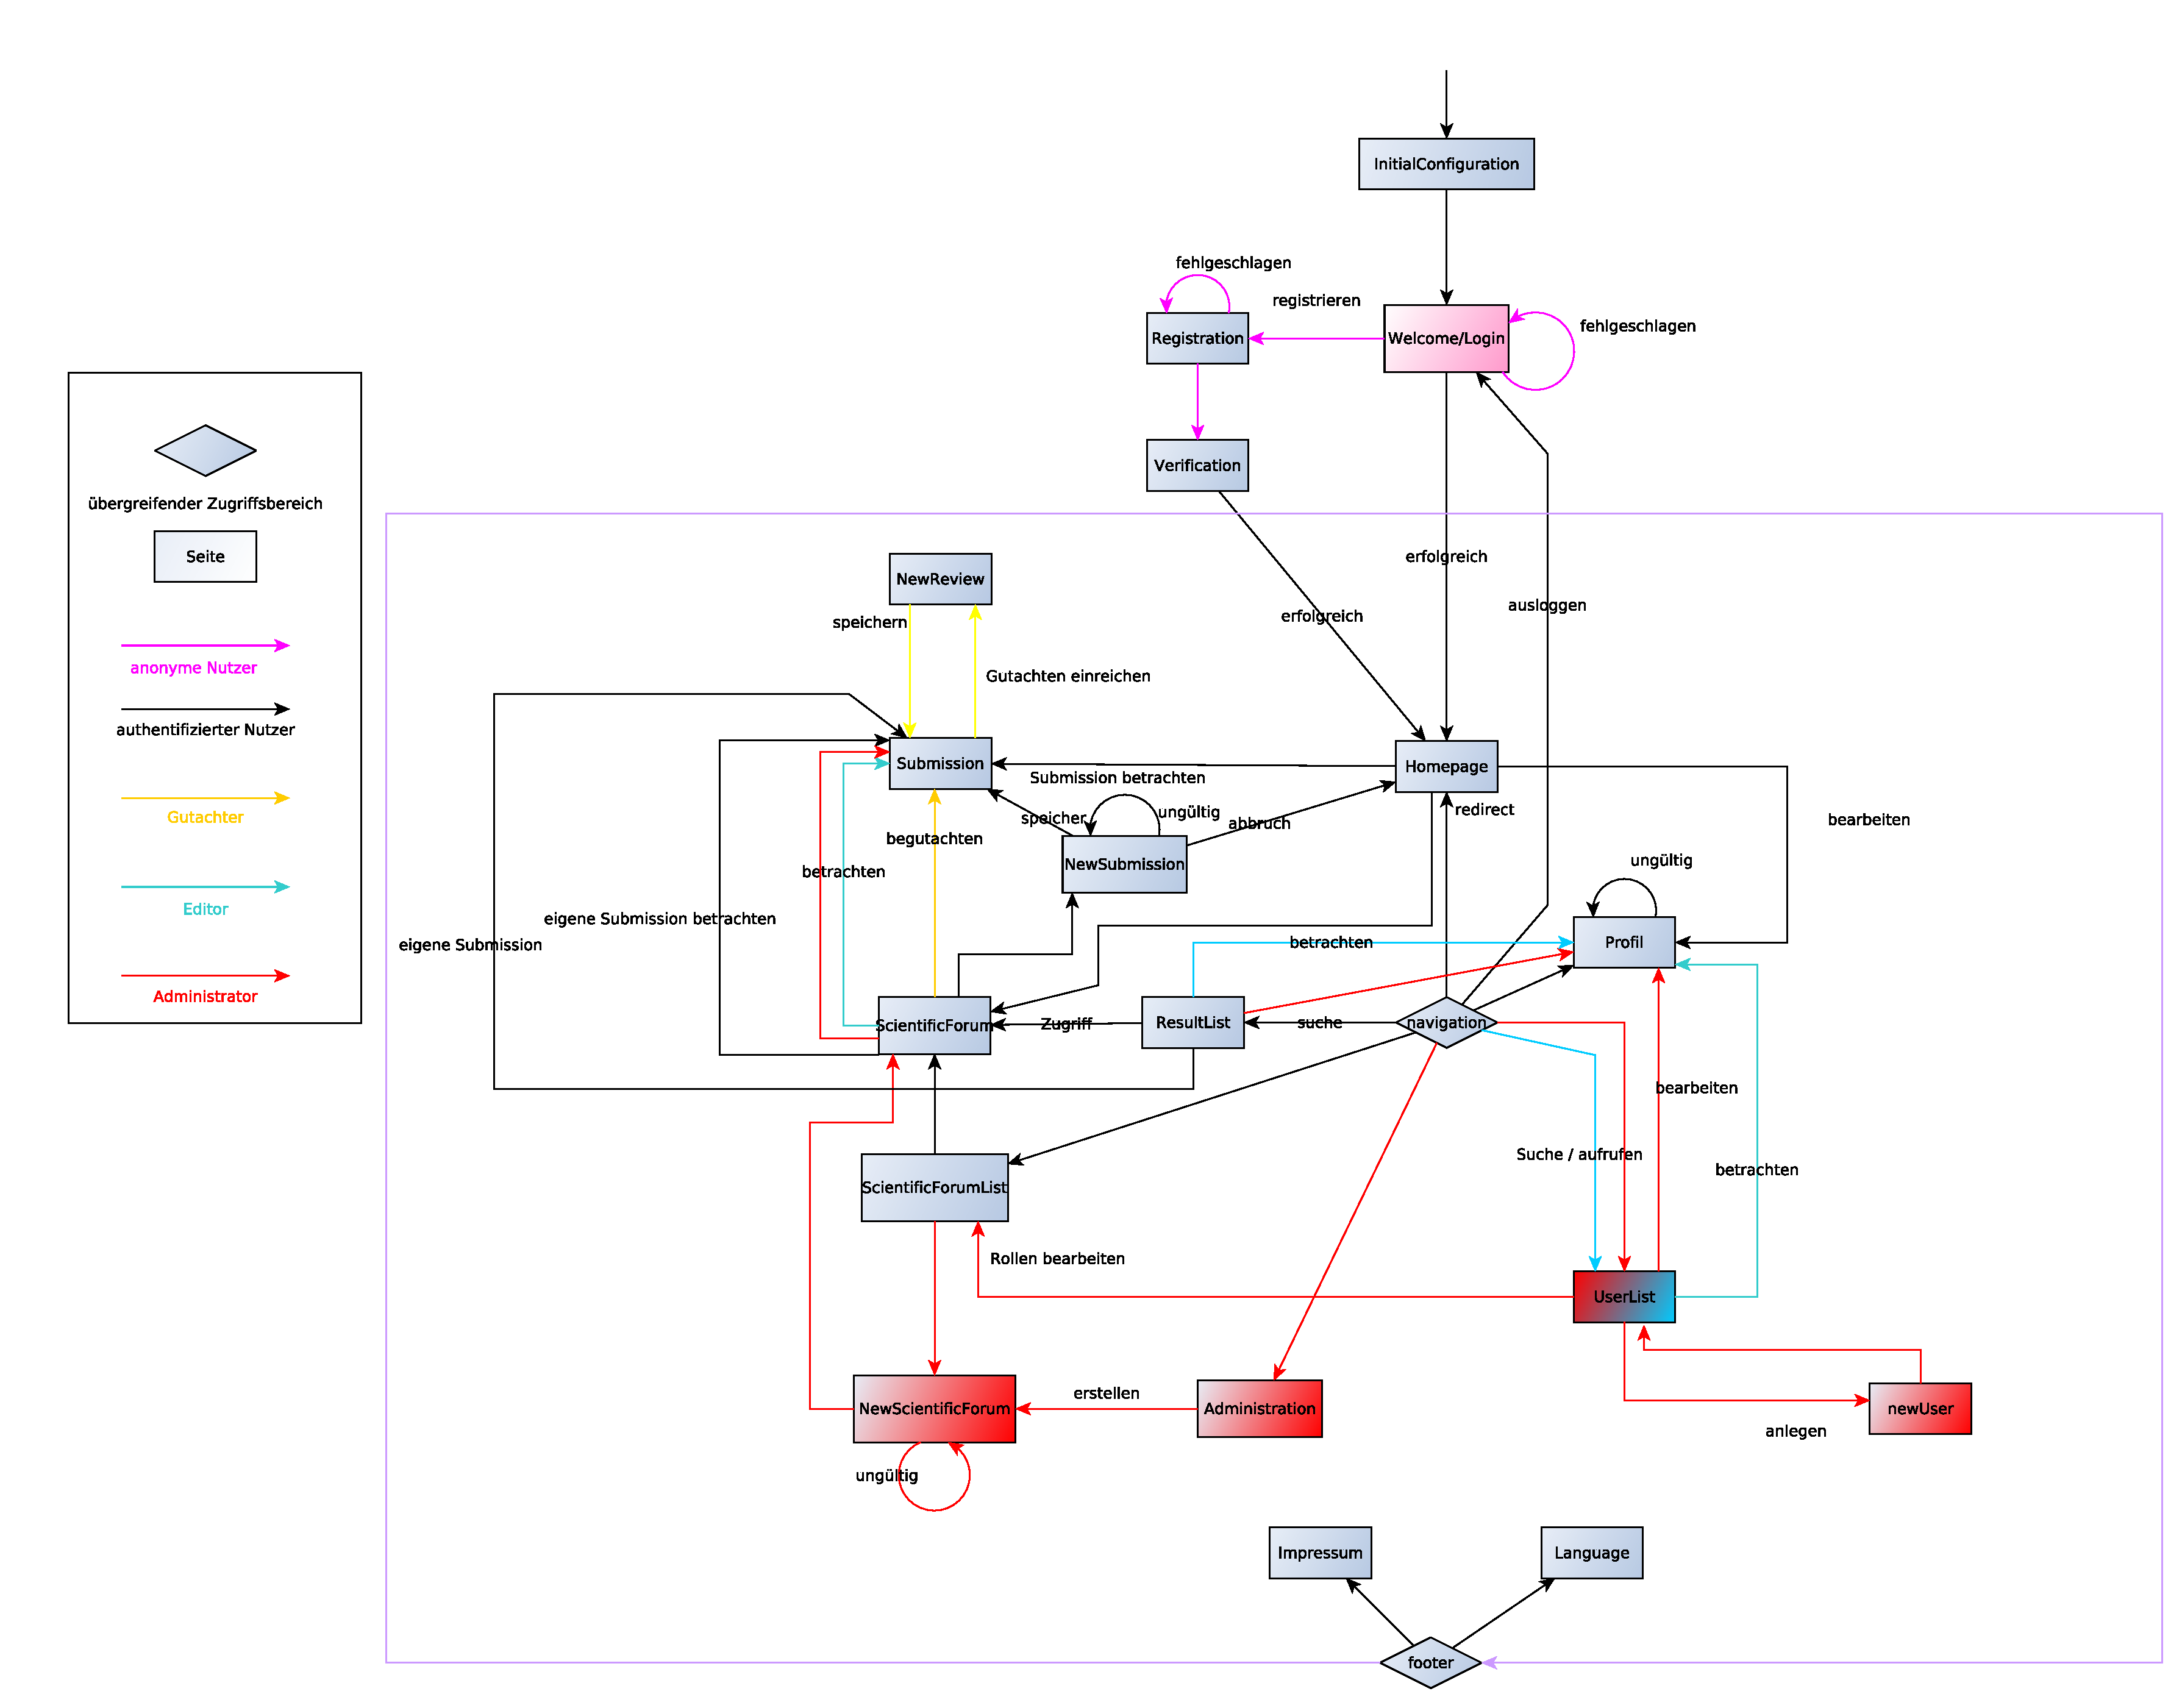
\includegraphics[width=\linewidth]{graphics/benutzerFlussyEd}
    \caption{Benutzerfluss}
	\label{fig:benutzerfluss}
\end{figure}

Die sich im Diagramm in Abbildung \ref{fig:benutzerfluss} befindlichen Rauten stellen Header (Navigationsleiste) und Footer dar.
Hierbei wird jedoch wie folgt unterschieden: Der Header ist nur für \hyperref[glo:regnutzer]{authentifizierte Nutzer} zugänglich,
d.h. dieser erscheint erst nach einem erfolgreichen Login und verschwindet nach dem Logout wieder.
Der Footer hingegen ist von jeder Seite der Applikation zugänglich und somit immer sichtbar.

Im Diagramm werden \hyperref[glo:admin]{Administratoren}, \hyperref[glo:editor]{Editoren}, \hyperref[glo:gutachter]{Gutachter} und normale Nutzende unter dem allgemeinen Begriff
authentifizierte Nutzer betrachtet.
Sind die Verbindungspfeile nicht schwarz, sondern andersfarbig dargestellt, so besitzen auch nur die
dargestellten Benutzergruppen ein Zugriffsrecht oder das Recht auf eine Aktion. (Administratoren von dieser Regelung
ausgeschlossen)

Des Weiteren ist der Randfall zu betrachten, bei welchem ein externer Gutachter, welcher noch nicht registriert ist,
eine Einladung eines Editors angenommen hat.
Diesem wird die Rolle eines Gutachters zugewiesen, jedoch besitzt er erst Zugriffsrechte, nachdem er sich
authentifiziert hat.